%
% bars.tex
%
\renewcommand{\thisname}{Chart::Bars}
\section{\thisname}
\name{\thisname}
\file{Bars.pm}
\requires{Chart::Base, GD, Carp, FileHandle}
\begin{Description}
The class \thisclass creates a chart made up of vertical bars.
\thisclass is a subclass of \class{Chart::Base}.
\end{Description}

\example
\begin{figure}[ht]
  \begin{center}
    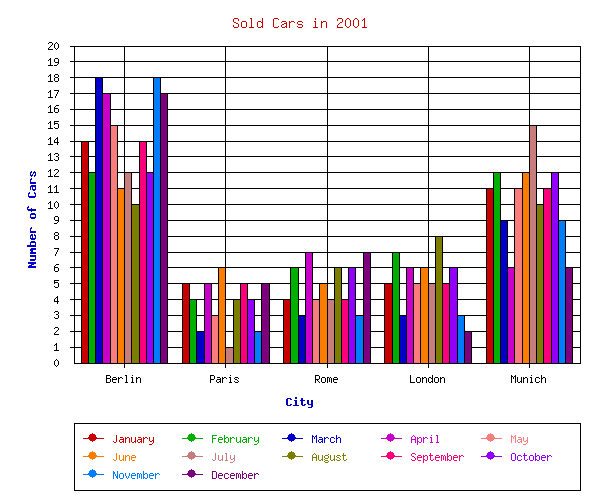
\includegraphics[scale=0.4]{d_bars.png}
  \end{center}
  \caption{Bar chart}
  \label{fig:bars}
\end{figure}

{\small
\begin{verbatim}
use Chart::Bars;

$g = Chart::Bars->new(600,500);

$g->add_dataset('Berlin', 'Paris', 'Rome', 'London', 'Munich');
$g->add_dataset(14, 5, 4, 5, 11);
$g->add_dataset(12, 4, 6, 7, 12);
$g->add_dataset(18, 2, 3, 3, 9);
$g->add_dataset(17, 5, 7, 6, 6);
$g->add_dataset(15, 3, 4, 5, 11);
$g->add_dataset(11, 6, 5, 6, 12);
$g->add_dataset(12, 1, 4, 5, 15);
$g->add_dataset(10, 4, 6, 8, 10);
$g->add_dataset(14, 5, 4, 5, 11);
$g->add_dataset(12, 4, 6, 6, 12);
$g->add_dataset(18, 2, 3, 3, 9);
$g->add_dataset(17, 5, 7, 2, 6);

%hash = ('title' => 'Sold Cars in 2001',
         'text_space'         => 5,
         'grey_background'    => 'false',
         'integer_ticks_only' => 'true',
         'x_label'            => 'City',
         'y_label'            => 'Number of Cars',
         'legend'             => 'bottom',
         'legend_labels'      => ['January',  'February', 
                                  'March',    'April',
                                  'May',      'June', 
                                  'July',     'August',
                                  'September','October', 
                                  'November', 'December'
                                 ],
         'min_val'            => 0,
         'max_val'            => 20,
         'grid_lines'         =>'true',
         'colors'             => {'title'   => 'red',
                                  'x_label' => 'blue',
                                  'y_label' => 'blue'
                                 }
        );

$g->set(%hash);

$g->png("bars.png");
\end{verbatim}
}

\constructorblurb{\thisname}

\begin{AttrDecl}{spaced\_bars}
Leaves some space between each group of bars when set to \literal{true}.
This usually make it easier to read a bar chart. Default is
\literal{true}.
\end{AttrDecl}

\begin{AttrDecl}{y\_axes}
Tells \thisclass where to place the $y$ axis. Valid values are
\literal{left}, \literal{right} and \literal{both}. Defaults to
\literal{left}.
\end{AttrDecl}
